% Options for packages loaded elsewhere
\PassOptionsToPackage{unicode}{hyperref}
\PassOptionsToPackage{hyphens}{url}
%
\documentclass[
  14pt,
  ignorenonframetext,
  aspectratio=169,
]{beamer}
\usepackage{pgfpages}
\setbeamertemplate{caption}[numbered]
\setbeamertemplate{caption label separator}{: }
\setbeamercolor{caption name}{fg=normal text.fg}
\beamertemplatenavigationsymbolsempty
% Prevent slide breaks in the middle of a paragraph
\widowpenalties 1 10000
\raggedbottom

\usepackage{amsmath,amssymb}
\usepackage{iftex}
\ifPDFTeX
  \usepackage[T1]{fontenc}
  \usepackage[utf8]{inputenc}
  \usepackage{textcomp} % provide euro and other symbols
\else % if luatex or xetex
  \usepackage{unicode-math}
  \defaultfontfeatures{Scale=MatchLowercase}
  \defaultfontfeatures[\rmfamily]{Ligatures=TeX,Scale=1}
\fi
\usepackage{lmodern}
\usetheme[]{monash}
\ifPDFTeX\else  
    % xetex/luatex font selection
\fi
% Use upquote if available, for straight quotes in verbatim environments
\IfFileExists{upquote.sty}{\usepackage{upquote}}{}
\IfFileExists{microtype.sty}{% use microtype if available
  \usepackage[]{microtype}
  \UseMicrotypeSet[protrusion]{basicmath} % disable protrusion for tt fonts
}{}
\makeatletter
\@ifundefined{KOMAClassName}{% if non-KOMA class
  \IfFileExists{parskip.sty}{%
    \usepackage{parskip}
  }{% else
    \setlength{\parindent}{0pt}
    \setlength{\parskip}{6pt plus 2pt minus 1pt}}
}{% if KOMA class
  \KOMAoptions{parskip=half}}
\makeatother
\usepackage{xcolor}
\newif\ifbibliography
\setlength{\emergencystretch}{3em} % prevent overfull lines
\setcounter{secnumdepth}{-\maxdimen} % remove section numbering


\providecommand{\tightlist}{%
  \setlength{\itemsep}{0pt}\setlength{\parskip}{0pt}}\usepackage{longtable,booktabs,array}
\usepackage{calc} % for calculating minipage widths
\usepackage{caption}
% Make caption package work with longtable
\makeatletter
\def\fnum@table{\tablename~\thetable}
\makeatother
\usepackage{graphicx}
\makeatletter
\def\maxwidth{\ifdim\Gin@nat@width>\linewidth\linewidth\else\Gin@nat@width\fi}
\def\maxheight{\ifdim\Gin@nat@height>\textheight\textheight\else\Gin@nat@height\fi}
\makeatother
% Scale images if necessary, so that they will not overflow the page
% margins by default, and it is still possible to overwrite the defaults
% using explicit options in \includegraphics[width, height, ...]{}
\setkeys{Gin}{width=\maxwidth,height=\maxheight,keepaspectratio}
% Set default figure placement to htbp
\makeatletter
\def\fps@figure{htbp}
\makeatother

% Colors
\definecolor{shadecolor}{RGB}{225,225,225}
\definecolor{DarkBrown}{RGB}{80,70,60}
\setbeamercolor{description item}{fg=Orange}
\setbeamercolor{block title alerted}{fg=white,bg=DarkBrown}
\setbeamercolor{block title}{fg=white,bg=DarkBrown}
\setbeamercolor{frametitle}{bg=DarkBrown,fg=white}

% Packages
\usepackage{amsmath, bm, amssymb, amsthm, mathrsfs,pifont,accents}
%\usepackage{enumitem,calc}
\usepackage[bb=boondox]{mathalfa}
\usepackage{url}
\usepackage{multirow, booktabs, float, textcmds, siunitx,multicol}
\usepackage{bm,booktabs,animate,ragged2e,multicol,microtype,hyperref}
\DeclareUnicodeCharacter{03BC}{$\mu$}
\usepackage{tikz}
\usetikzlibrary{calc}

% Figures
\graphicspath{{figs/}{tourism/}{energy/}}
\def\full#1{\vspace*{0.05cm}\centerline{\includegraphics[width=15cm,height=7.5cm,keepaspectratio=true]{#1}}}

% Fonts
\fontsize{13}{15}\sf
\usepackage[scale=0.85]{sourcecodepro}
\DisableLigatures{encoding = T1, family = tt*}
\usepackage{fontawesome5}

% Monash title page
\setbeamertemplate{title page}
{\placefig{5.}{-0.01}{width=1.01\paperwidth,height=1.01\paperheight}{figs/SWAS-ambo}
\placefig{0.4}{7.6}{width=4cm}{monash_bw}
\begin{textblock}{4.2}(.4,0.3)
\fontsize{16}{20}\selectfont\bfseries\sffamily\textcolor[RGB]{204,89,0}{\inserttitle}\\[0.3cm]
\fontsize{12}{12}\selectfont\bfseries\sffamily\textcolor[RGB]{204,89,0}{\insertsubtitle}
\end{textblock}
\begin{textblock}{7.5}(.4,6.2)
\fontsize{12}{13}\selectfont\sffamily\textcolor[RGB]{80,70,60}{\insertauthor}
\end{textblock}
\begin{textblock}{4.3}(.4,8.3)\pgfsetfillopacity{0.75}
\begin{beamercolorbox}[wd=4.3cm,ht=0.35cm,dp=0.2cm]{block body}
\fontsize{10}{10}\sf\color[RGB]{80,70,60}~\texttt{\href{https://robjhyndman.com/asc2023}{robjhyndman.com/asc2023}}
\end{beamercolorbox}
%\begin{beamerboxesrounded}[lower=block body, upper=block body]{}
%\fontsize{10}{10}\sf\color[RGB]{72,45,34}~\texttt{robjhyndman.com/isf2020}
%\end{beamerboxesrounded}
\end{textblock}
\begin{textblock}{6.2}(11.75,8.8)\pgfsetfillopacity{0.65}
\begin{beamercolorbox}[wd=4.2cm]{block body}
\fontsize{6}{6}\sf\color[RGB]{72,45,34}~Photo by \href{https://commons.wikimedia.org/wiki/File:SWAS-ambo-shout.jpg}{Graham Richardson} on \href{https://commons.wikimedia.org/wiki/File:SWAS-ambo-shout.jpg}{Wikimedia}
\end{beamercolorbox}
\end{textblock}}

%\renewenvironment{Shaded}{\color{black}\begin{snugshade}\color{black}}{\end{snugshade}\columnbreak}

% Tikz plots
\usetikzlibrary{trees,shapes,arrows,matrix,shadows,positioning}
\tikzstyle{decision} = [diamond, draw, fill=blue!20,
    text width=4.5em, text badly centered, node distance=4cm, inner sep=0pt]
\tikzstyle{block} = [rectangle, draw, fill=blue!20,
    text width=5cm, text centered, rounded corners, minimum height=4em]
\tikzstyle{line} = [draw, thick, -latex']
\tikzstyle{cloud} = [draw, ellipse,fill=red!20, node distance=3cm,
    minimum height=2em, text centered]
\tikzstyle{connector} = [->,thick]

\tikzset{
  basic/.style  = {draw, text width=2cm, font=\sffamily, rectangle},
  root/.style   = {basic, text width=3cm, rounded corners=2pt, thin, align=center, fill=red!30},
  level 2a/.style = {basic, rounded corners=2pt, thin,align=center, fill=blue!50, text width=7em},
  level 2b/.style = {basic, rounded corners=2pt, thin,align=center, fill=green!50, text width=7em},
  level 3a/.style = {basic, rounded corners=2pt, thin, align=center, fill=blue!30, text width=4em},
  level 3b/.style = {basic, rounded corners=2pt, thin, align=center, fill=green!30, text width=4em},
  level 4a/.style = {basic, rounded corners=2pt, thin, align=left, fill=blue!10, text width=3.5em},
  level 4b/.style = {basic, rounded corners=2pt, thin, align=left, fill=green!10, text width=3.5em}
}

% My definitions

\def\E{\text{E}}
\def\V{\text{Var}}
\def\bY{\bm{y}}
\def\by{\bm{y}}
\def\bS{\bm{S}}
\def\bG{\bm{G}}
\def\bI{\bm{I}}
\def\bJ{\bm{J}}
\def\bSigma{\bm{\Sigma}}
\def\bLambda{\bm{\Lambda}}
\def\Var{\text{Var}}
\def\var{\text{Var}}
\newcommand{\btwocol}{\begin{multicols}{2}}
\newcommand{\etwocol}{\end{multicols}}

% BIBLIOGRAPHIES
\usepackage[style=authoryear,bibencoding=utf8,minnames=1,maxnames=4, maxbibnames=99,natbib=true,dashed=false,terseinits=true,giveninits=true,uniquename=false,uniquelist=false,labeldate=true,doi=false, isbn=false, natbib=true,backend=biber]{biblatex}

\DeclareFieldFormat{url}{\url{#1}}
\DeclareFieldFormat[article]{pages}{#1}
\DeclareFieldFormat[inproceedings]{pages}{\lowercase{pp.}#1}
\DeclareFieldFormat[incollection]{pages}{\lowercase{pp.}#1}
\DeclareFieldFormat[article]{volume}{\mkbibbold{#1}}
\DeclareFieldFormat[article]{number}{\mkbibparens{#1}}
\DeclareFieldFormat[article]{title}{\MakeCapital{#1}}
\DeclareFieldFormat[article]{url}{}
\DeclareFieldFormat[Techreport]{Url}{}
\DeclareFieldFormat[book]{url}{}
\DeclareFieldFormat[inbook]{url}{}
\DeclareFieldFormat[incollection]{url}{}
\DeclareFieldFormat[inproceedings]{url}{}
\DeclareFieldFormat[inproceedings]{title}{#1}
\DeclareFieldFormat{shorthandwidth}{#1}
%\DeclareFieldFormat{extrayear}{}
% No dot before number of articles
\usepackage{xpatch}
\xpatchbibmacro{volume+number+eid}{\setunit*{\adddot}}{}{}{}
% Remove In: for an article.
\renewbibmacro{in:}{%
  \ifentrytype{article}{}{%
  \printtext{\bibstring{in}\intitlepunct}}}

\AtEveryBibitem{\clearfield{month}}
\AtEveryCitekey{\clearfield{month}}
\AtBeginBibliography{\fontsize{11}{11}\sf}
\setbeamertemplate{frametitle continuation}{}

\graphicspath{{figs/}}
\makeatletter
\@ifpackageloaded{caption}{}{\usepackage{caption}}
\AtBeginDocument{%
\ifdefined\contentsname
  \renewcommand*\contentsname{Table of contents}
\else
  \newcommand\contentsname{Table of contents}
\fi
\ifdefined\listfigurename
  \renewcommand*\listfigurename{List of Figures}
\else
  \newcommand\listfigurename{List of Figures}
\fi
\ifdefined\listtablename
  \renewcommand*\listtablename{List of Tables}
\else
  \newcommand\listtablename{List of Tables}
\fi
\ifdefined\figurename
  \renewcommand*\figurename{Figure}
\else
  \newcommand\figurename{Figure}
\fi
\ifdefined\tablename
  \renewcommand*\tablename{Table}
\else
  \newcommand\tablename{Table}
\fi
}
\@ifpackageloaded{float}{}{\usepackage{float}}
\floatstyle{ruled}
\@ifundefined{c@chapter}{\newfloat{codelisting}{h}{lop}}{\newfloat{codelisting}{h}{lop}[chapter]}
\floatname{codelisting}{Listing}
\newcommand*\listoflistings{\listof{codelisting}{List of Listings}}
\makeatother
\makeatletter
\makeatother
\makeatletter
\@ifpackageloaded{caption}{}{\usepackage{caption}}
\@ifpackageloaded{subcaption}{}{\usepackage{subcaption}}
\makeatother
\ifLuaTeX
  \usepackage{selnolig}  % disable illegal ligatures
\fi
\IfFileExists{bookmark.sty}{\usepackage{bookmark}}{\usepackage{hyperref}}
\IfFileExists{xurl.sty}{\usepackage{xurl}}{} % add URL line breaks if available
\urlstyle{same} % disable monospaced font for URLs
\hypersetup{
  pdftitle={Probabilistic Forecast Reconciliation For Emergency Services Demand},
  pdfauthor={Rob J HyndmanBahman Rostami-Tabar},
  hidelinks,
  pdfcreator={LaTeX via pandoc}}

\title{Probabilistic Forecast Reconciliation For Emergency Services
Demand}
\author{Rob J Hyndman\newline Bahman Rostami-Tabar}
\date{}

\begin{document}
\frame{\titlepage}

\begin{frame}{Wales Health Board Areas}
\phantomsection\label{wales-health-board-areas}
\placefig{3.3}{1.2}{width=7.8cm}{Map-of-Wales-Health-Boards}
\end{frame}

\begin{frame}{Data}
\phantomsection\label{data}
\begin{itemize}
\tightlist
\item
  Daily number of attended incidents:\newline 1 October 2015 -- 31 July
  2019
\item
  Disaggregated by:

  \begin{itemize}
  \tightlist
  \item
    control area
  \item
    health board
  \item
    priority
  \item
    nature of incidents
  \end{itemize}
\item
  2,142,000 rows observations from 1,530 time series.
\end{itemize}
\end{frame}

\begin{frame}{Data structure}
\phantomsection\label{data-structure}
\placefig{0.3}{1.5}{width=7cm}{group.pdf}
\placefig{7.5}{1.5}{width=7.7cm}{group.png}
\end{frame}

\begin{frame}{Data structure}
\phantomsection\label{data-structure-1}
\fontsize{10}{11}\sf

\begin{table}
\centering
\begin{tabular}{lr}
\toprule
Level & Number of series\\
\midrule
All country & 1\\
Control & 3\\
Health board & 7\\
Priority & 3\\
Priority * Control & 9\\
Priority * Health board & 21\\
Nature of incident & 35\\
Nature of incident * Control & 105\\
Nature of incident * Health board & 245\\
Priority * Nature of incident & 104\\
Control * Priority * Nature of incident & 306\\
Control * Health board * Priority * Nature of incident (Bottom level) & 691\\
Total & 1530\\
\bottomrule
\end{tabular}
\end{table}
\end{frame}

\begin{frame}[fragile]{Data}
\phantomsection\label{data-1}
\fontsize{10}{10}\sf

\begin{verbatim}
# A tsibble: 2,142,000 x 6 [1D]
# Key:       region, category, nature, lhb [1,530]
   date       region       category     nature       lhb          incident
   <date>     <chr*>       <chr*>       <chr*>       <chr*>          <dbl>
 1 2015-10-01 <aggregated> <aggregated> <aggregated> <aggregated>     1020
 2 2015-10-02 <aggregated> <aggregated> <aggregated> <aggregated>     1021
 3 2015-10-03 <aggregated> <aggregated> <aggregated> <aggregated>     1025
 4 2015-10-04 <aggregated> <aggregated> <aggregated> <aggregated>     1043
 5 2015-10-05 <aggregated> <aggregated> <aggregated> <aggregated>     1067
 6 2015-10-06 <aggregated> <aggregated> <aggregated> <aggregated>     1063
 7 2015-10-07 <aggregated> <aggregated> <aggregated> <aggregated>      973
 8 2015-10-08 <aggregated> <aggregated> <aggregated> <aggregated>     1057
 9 2015-10-09 <aggregated> <aggregated> <aggregated> <aggregated>     1026
10 2015-10-10 <aggregated> <aggregated> <aggregated> <aggregated>     1063
# i 2,141,990 more rows
\end{verbatim}
\end{frame}

\begin{frame}[fragile]{Data}
\phantomsection\label{data-2}
\fontsize{10}{10}\sf

\begin{verbatim}
# A tsibble: 2,142,000 x 6 [1D]
# Key:       region, category, nature, lhb [1,530]
   date       region category nature    lhb          incident
   <date>     <chr*> <chr*>   <chr*>    <chr*>          <dbl>
 1 2015-10-01 C      Amber    ABDOMINAL HD                  0
 2 2015-10-01 C      Amber    ABDOMINAL PO                  0
 3 2015-10-01 C      Amber    ABDOMINAL SB                  0
 4 2015-10-01 C      Amber    ABDOMINAL <aggregated>        0
 5 2015-10-01 C      Amber    ALLERGIES HD                  0
 6 2015-10-01 C      Amber    ALLERGIES PO                  1
 7 2015-10-01 C      Amber    ALLERGIES SB                  0
 8 2015-10-01 C      Amber    ALLERGIES <aggregated>        1
 9 2015-10-01 C      Amber    ANIMALBIT HD                  0
10 2015-10-01 C      Amber    ANIMALBIT PO                  0
# i 2,141,990 more rows
\end{verbatim}
\end{frame}

\begin{frame}{Aggregated daily incidents}
\phantomsection\label{aggregated-daily-incidents}
\vspace*{0.2cm}

\only<1>{\centerline{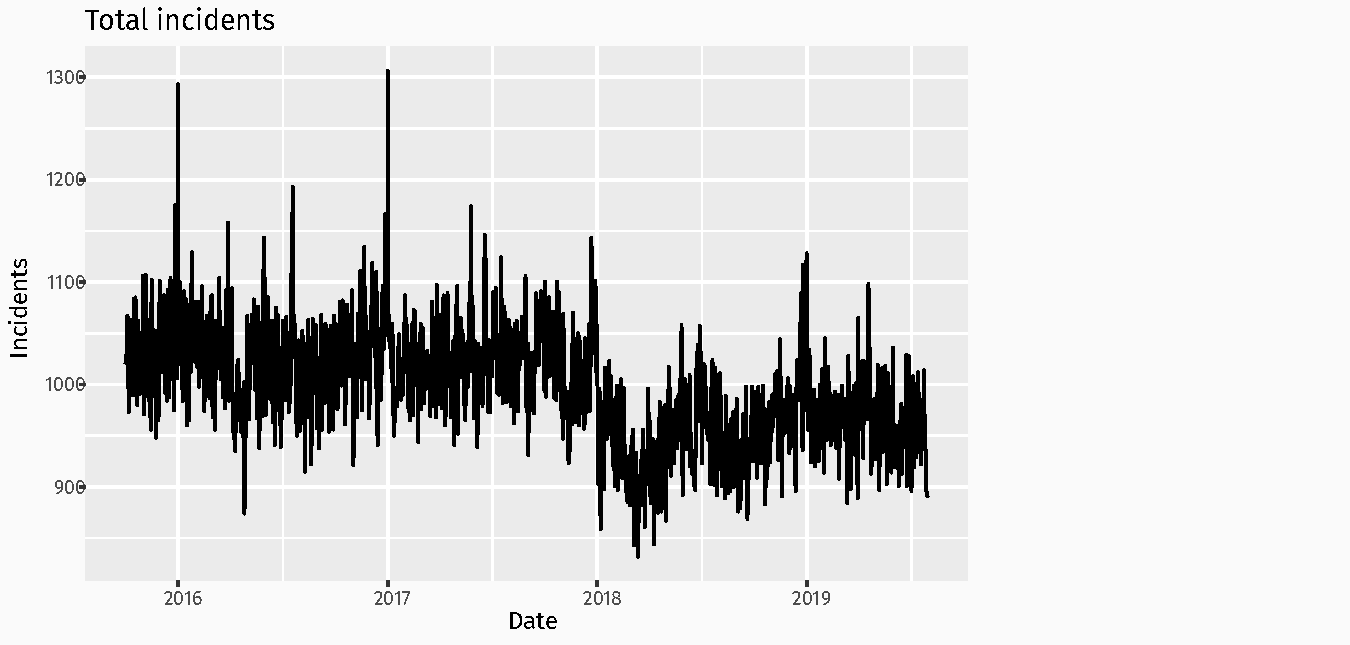
\includegraphics[width=15.8cm]{figs/time_plots1.pdf}}}
\only<2>{\centerline{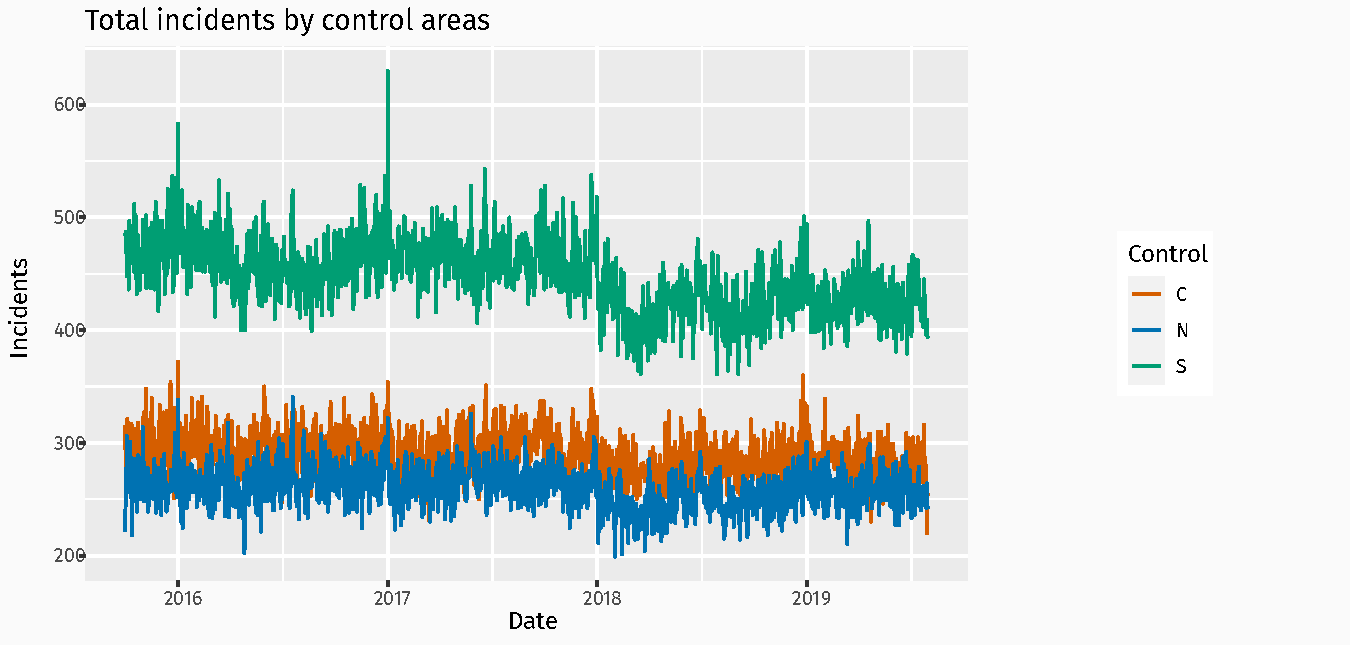
\includegraphics[width=15.8cm]{figs/time_plots2.pdf}}}
\only<3>{\centerline{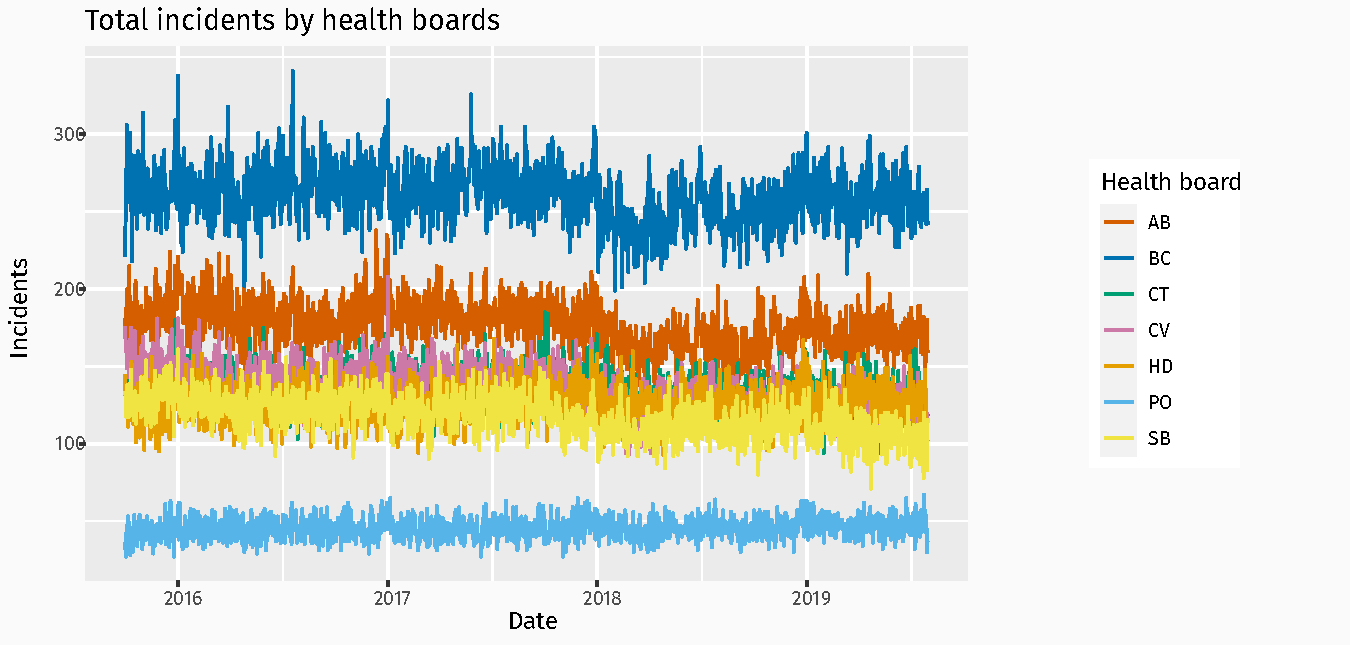
\includegraphics[width=15.8cm]{figs/time_plots3.pdf}}}
\only<4>{\centerline{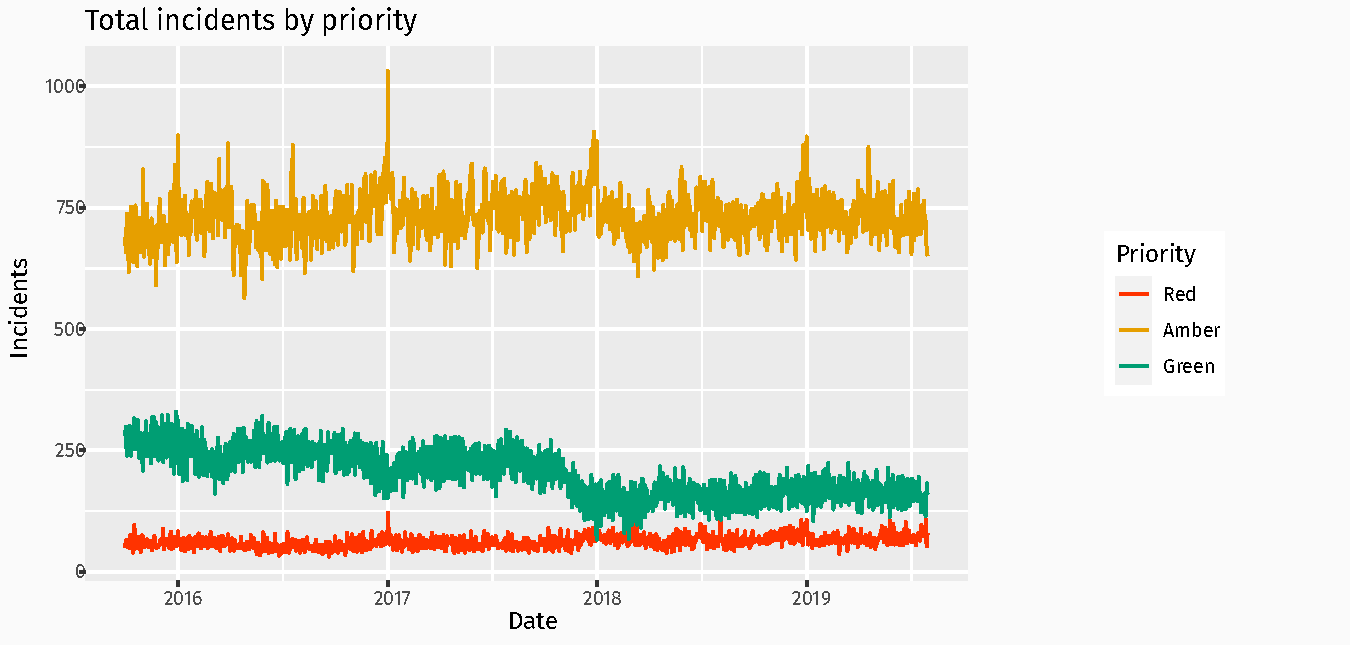
\includegraphics[width=15.8cm]{figs/time_plots4.pdf}}}
\only<5>{\centerline{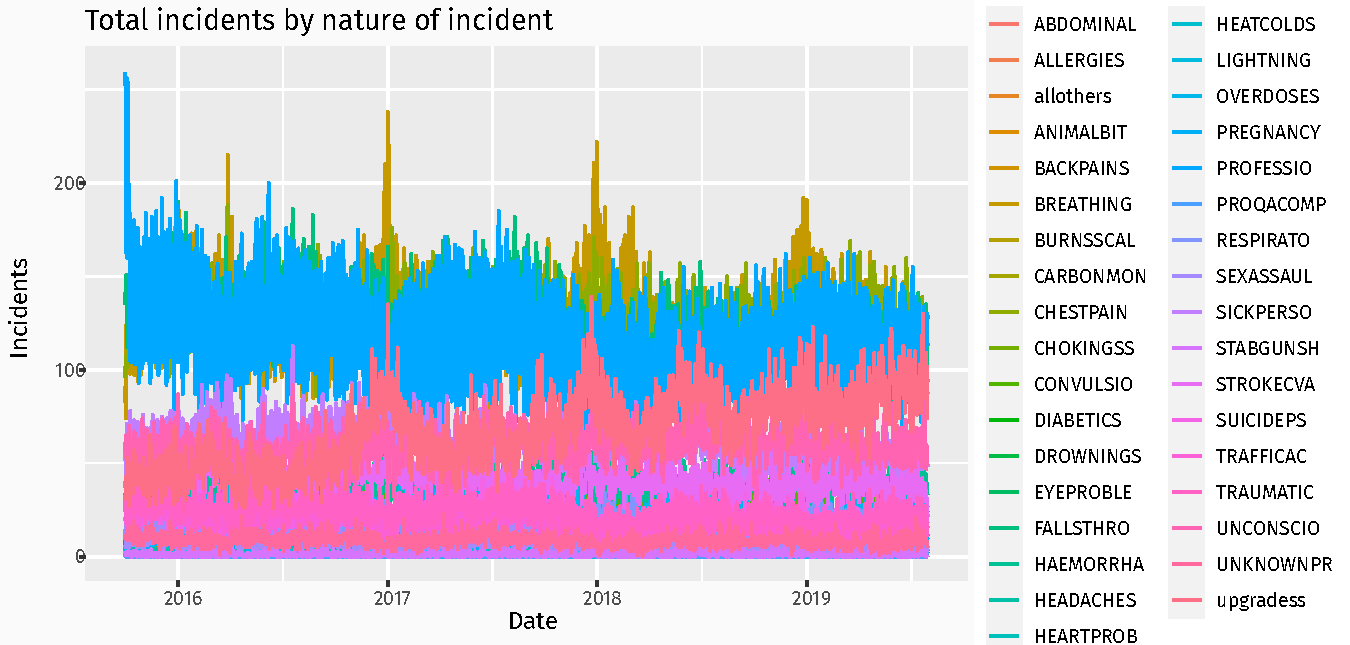
\includegraphics[width=15.8cm]{figs/time_plots5.pdf}}}
\only<6>{\centerline{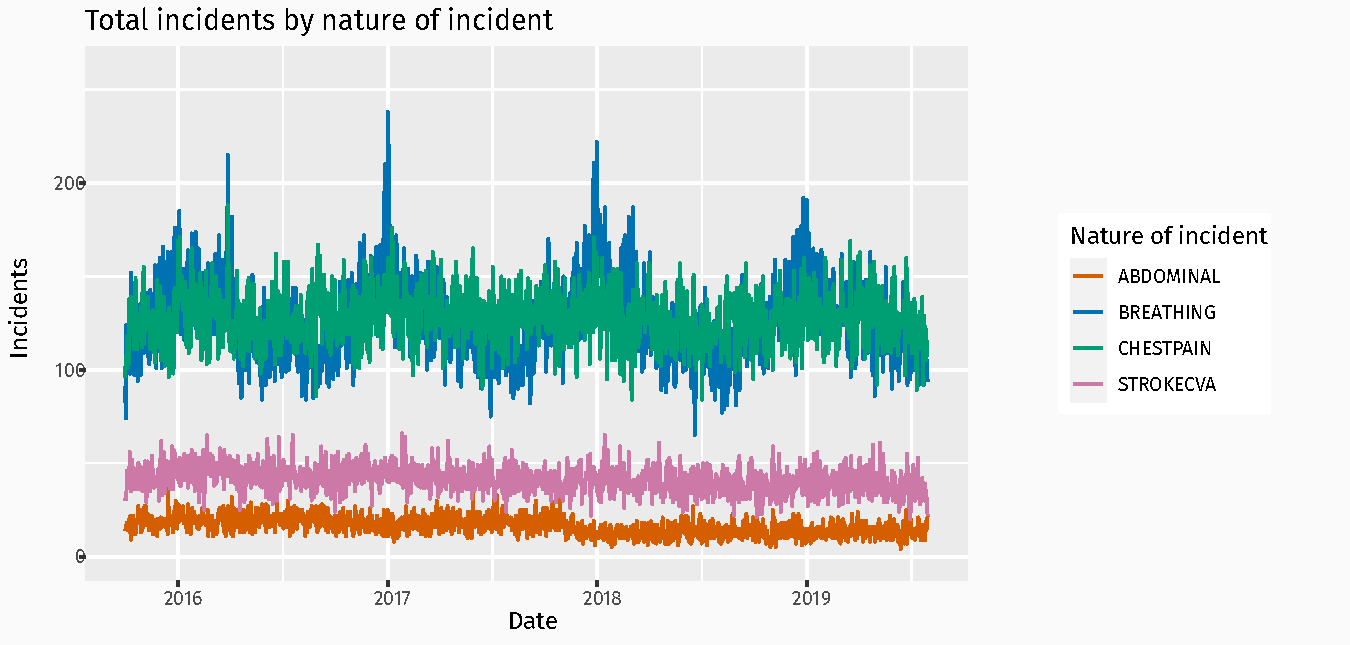
\includegraphics[width=15.8cm]{figs/time_plots6.pdf}}}
\end{frame}

\begin{frame}{Forecasting methods}
\phantomsection\label{forecasting-methods}
\begin{enumerate}
\tightlist
\item
  \textbf{Naïve}: Empirical distribution of past daily attended
  incidents.
\item
  \textbf{ETS}: Exponential Smoothing State Space models.
\item
  \textbf{GLM}: Poission Regression with spline trend, day of the week,
  annual Fourier seasonality, public holidays, school holidays,
  Christmas Day, New Year's Day.
\item
  \textbf{TSGLM}: Poisson Regression with same covariates plus three
  autoregressive terms.
\item
  \textbf{Ensemble}: Mixture distribution of 1--4.
\end{enumerate}
\end{frame}

\begin{frame}{Notation}
\phantomsection\label{notation}
\begin{textblock}{8.5}(0.2,1.5)
Every collection of time series with linear constraints can be written as
\centerline{\colorbox[RGB]{210,210,210}{$\bY_{t}=\color{blue}\bS\color{red}\bm{b}_{t}$}}
\vspace*{-0.9cm}\begin{itemize}\parskip=0cm\itemsep=0cm
\item $\by_t=$ vector of all series at time $t$
\item $ y_{\text{Total},t}= $ aggregate of all series at time
$t$.
\item $ y_{X,t}= $ value of series $X$ at time $t$.
\item $\color{red}{\bm{b}_t}=$ vector of most disaggregated series at time $t$
\item $\color{blue}{\bS}=$ ``summing matrix'' containing the linear constraints.
\end{itemize}
\end{textblock}

\begin{textblock}{5.7}(11.4,0.1)
\begin{minipage}{4cm}
\begin{block}{}\centering
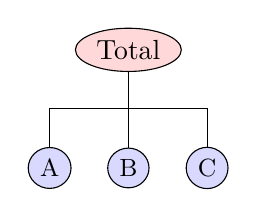
\begin{tikzpicture}
\tikzstyle{every node}=[ellipse,draw,fill=red!15,inner sep=2pt]
\tikzstyle[level distance=.3cm]
\tikzstyle[sibling distance=12cm]
\tikzstyle{level 1}=[sibling distance=10mm,font=\small,set style={{every node}+=[fill=blue!15]}]
\node{Total}[edge from parent fork down]
 child {node {A}
 }
 child {node {B}
 }
 child {node {C}
 };
\end{tikzpicture}
\end{block}
\end{minipage}
\end{textblock}

\only<1>{\begin{textblock}{5.7}(9.4,2.8)\fontsize{14}{15}\sf
\begin{align*}
\bY_{t}&= \begin{pmatrix}
  y_{\text{Total},t}\\
  y_{A,t}\\
  y_{B,t}\\
  y_{C,t}
  \end{pmatrix}  \\
  &= {\color{blue}\underbrace{\begin{pmatrix}
                1 & 1 & 1 \\
                1 & 0 & 0 \\
                0 & 1 & 0\\
                0 & 0 & 1
                \end{pmatrix}}_{\bS}}
     {\color{red}\underbrace{\begin{pmatrix}
       y_{A,t}\\y_{B,t}\\y_{C,t}
       \end{pmatrix}}_{\bm{b}_{t}}}
\end{align*}
\end{textblock}}
\only<2>{\begin{textblock}{5.7}(9.4,3.2)\fontsize{14}{15}\sf
\begin{alertblock}{}
\begin{itemize}\itemsep=0.1cm
\item Base forecasts: $\hat{\bm{y}}_{T+h|T}$
\item Reconciled forecasts: $\tilde{\bm{y}}_{T+h|T}=\bS\bm{G}\hat{\bm{y}}_{T+h|T}$
\item MinT: $\bG = (\bS'\bm{W}_h^{-1}\bS)^{-1}\bS'\bm{W}_h^{-1}$ where $\bm{W}_h$ is covariance matrix of base forecast errors.
\end{itemize}
\end{alertblock}
\end{textblock}}
\end{frame}

\begin{frame}{Nonparametric bootstrap reconciliation}
\phantomsection\label{nonparametric-bootstrap-reconciliation}
\begin{itemize}
\tightlist
\item
  Fit model to all series and store the residuals as
  \(\underaccent{\tilde}{\bm{\varepsilon}}_t\).
\item
  These should be serially uncorrelated but cross-sectionally
  correlated.
\item
  Draw iid samples from
  \(\underaccent{\tilde}{\bm{\varepsilon}}_1,\dots,\underaccent{\tilde}{\bm{\varepsilon}}_T\)
  with replacement.
\item
  Simulate future sample paths for model using the bootstrapped
  residuals.
\item
  Reconcile each sample path using MinT.
\item
  Combine the reconciled sample paths to form a mixture distribution at
  each forecast horizon.
\end{itemize}
\end{frame}

\begin{frame}{Boostrapping residuals}
\phantomsection\label{boostrapping-residuals}
\vspace*{0.2cm}
\centerline{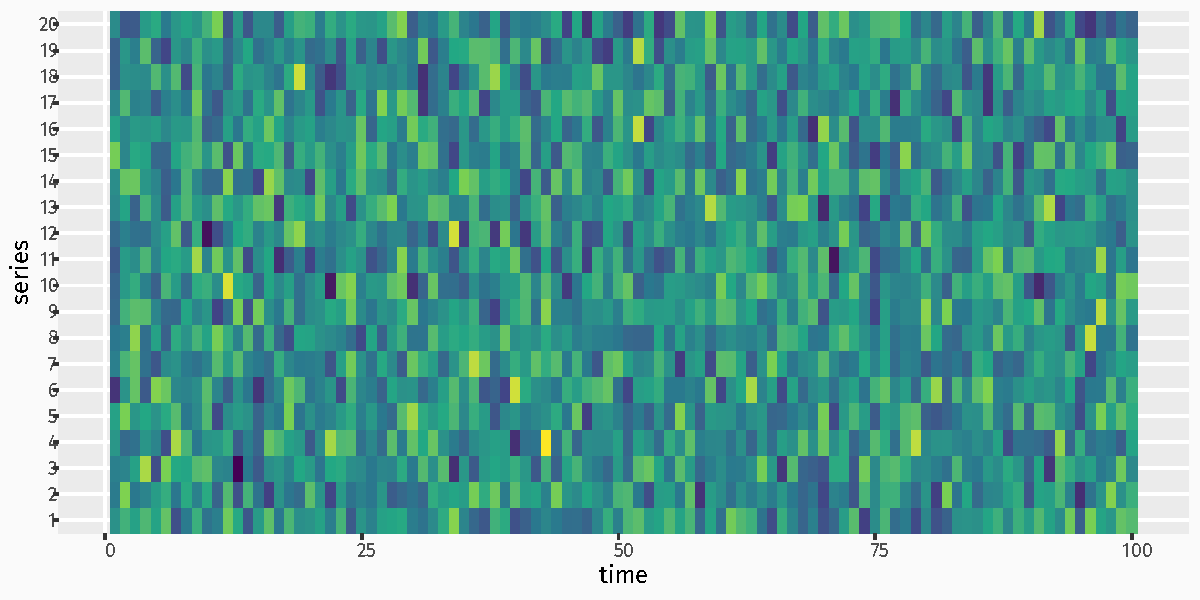
\includegraphics[width=15.5cm]{figs/sim_bootstrap.pdf}}
\end{frame}

\begin{frame}{Boostrapping residuals}
\phantomsection\label{boostrapping-residuals-1}
\vspace*{0.2cm}
\centerline{
\animategraphics[loop,autoplay,width=15.5cm]{10}{figs/sim_bootstrap_}{1}{20}
}
\end{frame}

\begin{frame}{Performance evaluation}
\phantomsection\label{performance-evaluation}
\begin{itemize}
\tightlist
\item
  Ten-fold time series cross-validation
\item
  Forecast horizon of 1--84 days
\item
  Each training set contains an additional 42 days.
\item
  Forecasts at 43--84 days correspond to planning horizon.
\end{itemize}

\includegraphics{asc2023_files/figure-beamer/cv1-1.pdf}
\end{frame}

\begin{frame}{Forecast accuracy: 43--84 days ahead}
\phantomsection\label{forecast-accuracy-4384-days-ahead}
\fontsize{10}{12}\sf

\begin{tabular}[t]{llrrr}
\toprule
\multicolumn{2}{c}{ } & \multicolumn{3}{c}{MSSE} \\
\cmidrule(l{3pt}r{3pt}){3-5}
Method & Model & Total & Control areas & Health boards\\
\midrule
Base & Naïve & 1.169 & 1.056 & 1.062\\
Base & ETS & 0.979 & 0.875 & 0.816\\
Base & GLM & 0.813 & 0.897 & 0.875\\
Base & TSGLM & 0.822 & 0.901 & 0.875\\
Base & Ensemble & 0.599 & 0.729 & 0.774\\
\addlinespace
MinT & Naïve & 1.168 & 1.057 & 1.062\\
MinT & ETS & 0.785 & 0.852 & 0.845\\
MinT & GLM & 0.720 & 0.827 & 0.837\\
MinT & TSGLM & 0.722 & 0.833 & 0.839\\
MinT & Ensemble & \textbf{0.560} & \textbf{0.706} & \textbf{0.765}\\
\bottomrule
\end{tabular}

\begin{textblock}{4.2}(11.6, 1.2)
\begin{block}{}
\centerline{$\text{MSSE} = \text{mean}(q_{j}^2)$}
$$
  q^2_{j} = \frac{ e^2_{j}}
 {\displaystyle\frac{1}{T-7}\sum_{t=8}^T (y_{t}-y_{t-7})^2}
$$
\begin{itemize}
\item Observations: $y_1,\dots,y_T$.
\item Forecast errors: $e_{j}=y_{T+j}-\hat{y}_{T+j|T}$.
\end{itemize}
\end{block}
\end{textblock}
\end{frame}

\begin{frame}{Forecast accuracy: 43--84 days ahead}
\phantomsection\label{forecast-accuracy-4384-days-ahead-1}
\fontsize{10}{12}\sf

\begin{tabular}[t]{llrrr}
\toprule
\multicolumn{2}{c}{ } & \multicolumn{3}{c}{CRPS} \\
\cmidrule(l{3pt}r{3pt}){3-5}
Method & Model & Total & Control areas & Health boards\\
\midrule
Base & Naïve & 30.387 & 10.882 & 5.500\\
Base & ETS & 14.309 & 6.074 & 3.476\\
Base & GLM & 15.396 & 6.253 & 3.576\\
Base & TSGLM & 15.316 & 6.227 & 3.575\\
Base & Ensemble & 12.978 & \textbf{5.727} & 3.430\\
\addlinespace
MinT & Naïve & 30.368 & 10.902 & 5.498\\
MinT & ETS & 13.515 & 5.967 & 3.547\\
MinT & GLM & 13.839 & 5.917 & 3.453\\
MinT & TSGLM & 14.000 & 5.947 & 3.455\\
MinT & Ensemble & \textbf{12.585} & 5.728 & \textbf{3.426}\\
\bottomrule
\end{tabular}

\begin{textblock}{4.2}(11.6, 1.2)
\begin{block}{}
\centerline{$\text{CRPS} = \text{mean}(p_j)$}
$$
  p_j = \int_{-\infty}^{\infty} \left(G_j(x) - F_j(x)\right)^2dx,
$$
\begin{itemize}
\item $G_j(x)=$ forecast distribution for forecast horizon $j$
\item $F_j(x)=$ empirical distribution for same period
\end{itemize}
\end{block}
\end{textblock}
\end{frame}

\begin{frame}{Conclusions}
\phantomsection\label{conclusions}
\begin{itemize}
\tightlist
\item
  Ensemble mixture distributions give better forecasts than any
  component methods.
\item
  Forecast reconciliation improves forecast accuracy, even when some
  component methods are quite poor.
\item
  The ensemble without the Naïve method was worse.
\item
  Forecast reconciliation allows coordinated planning and resource
  allocation.
\end{itemize}

\only<2>{\begin{textblock}{14}(.9,6.8)
\begin{block}{}
\fontsize{13}{14}\sf
\begin{multicols}{2}
\begin{itemize}\parskip = 0cm\itemsep = 0.2cm
\item[\faIcon{chalkboard-teacher}] \href{https://robjhyndman.com/asc2023}{robjhyndman.com/asc2023}
\item[{\faIcon[regular]{file-alt}}] \href{https://robjhyndman.com/fems}{robjhyndman.com/fems}
\item[\faIcon{mastodon}] \href{https://aus.social/@robjhyndman}{aus.social/@robjhyndman}
\item[\faIcon{envelope}] \href{mailto:rob.hyndman@monash.edu}{rob.hyndman@monash.edu}
\end{itemize}
\end{multicols}
\end{block}
\end{textblock}}
\end{frame}



\end{document}
